\chapter{Prototype}
\label{chap:prototype}

\begin{chapterintro}

In this chapter, we will describe the prototype we developed following the architecture described in the previous chapter.
 
\end{chapterintro}

\cleardoublepage

\section{Overview of the system}

For this system, we developed a prototype utilising the architecture explained in chapter \ref{chap:architecture}. To do so, we deployed the following modules and subsystems:

\begin{enumerate}
 \item A Javascript client, that will connect to the system and act as an user interface.
 \item A Front-end controller, written in python, that will handle the interaction between the different modules-
 \item A chatbot using chatscript, to handle question analysis and chit-chat interaction.
 \item An Apache Solr instance, where all the semantic data will be loaded.
\end{enumerate}

In parallel to all this, both a web scraper using scrapy to recover the relevant data, and an uploader to post the data to Solr.

\subsection{Chat client}
\label{sec:chatclient}

In our prototype, the interaction with the system is done via a web client that provides a chat box and an iframe where the content is located. When the user first opens the page, it's greeted by the bot, and provided with a   short explanation of how the client works.

\begin{figure}[!htbp]
    \centering
    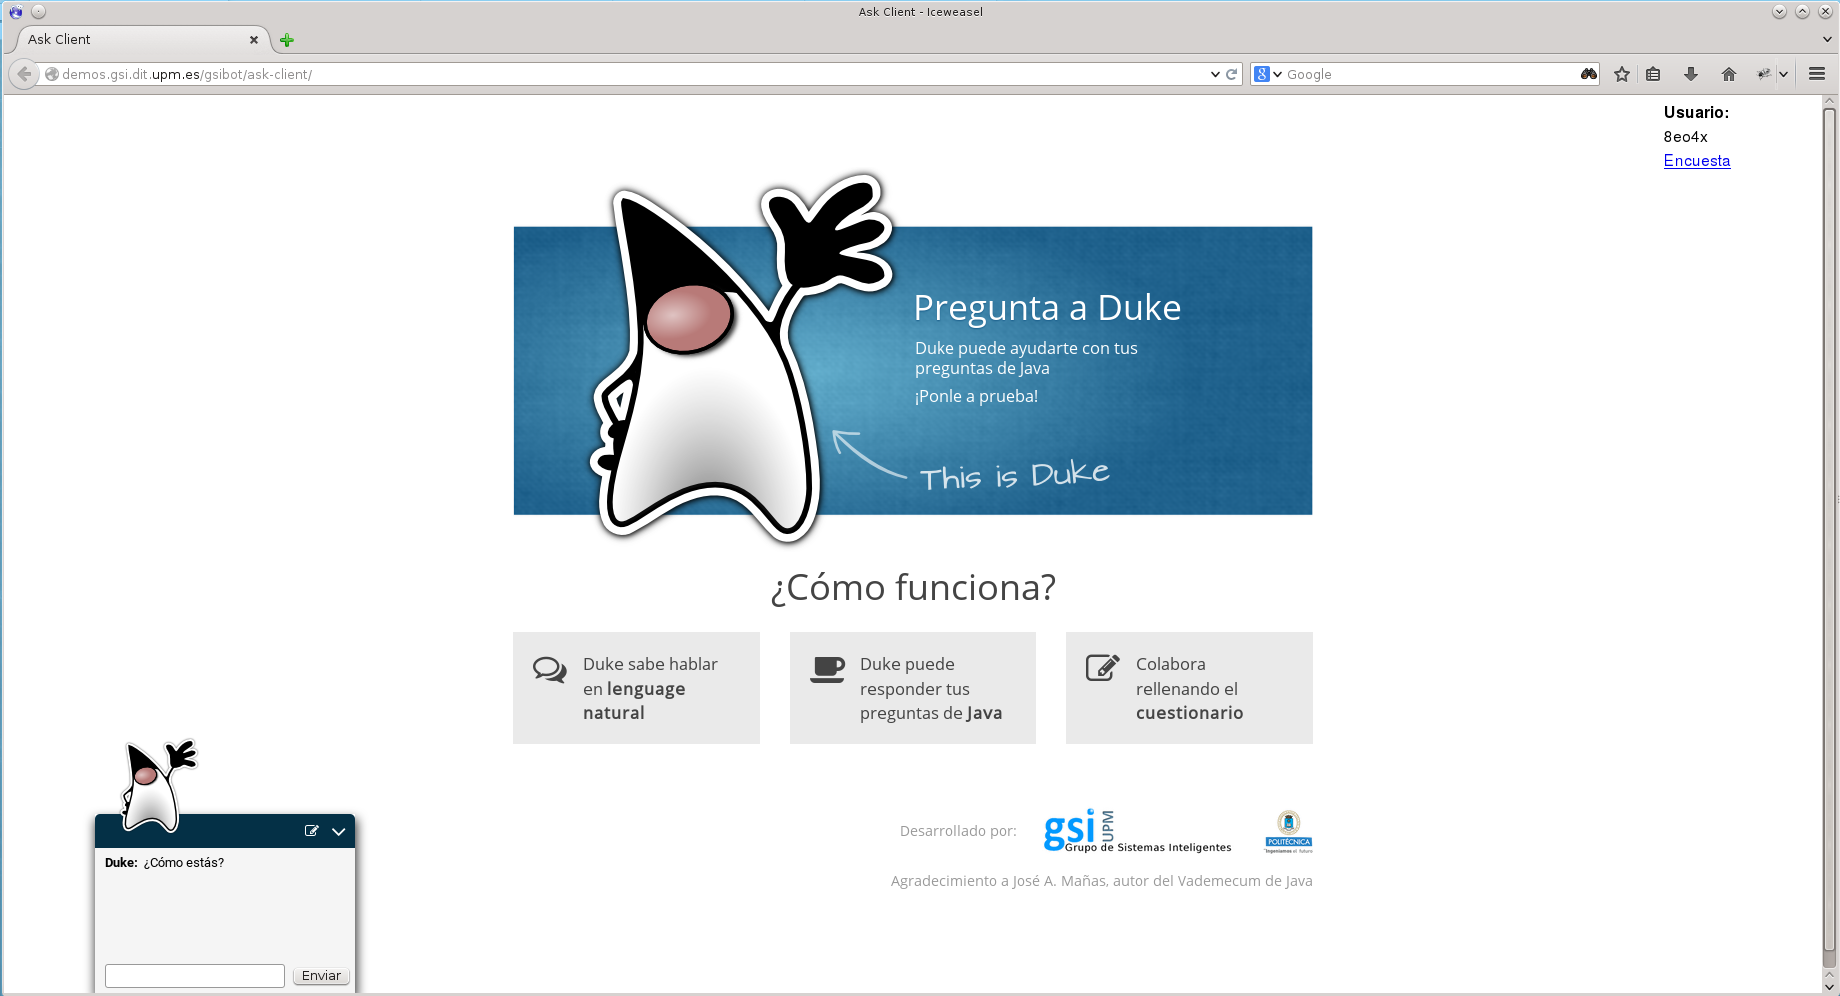
\includegraphics[width=0.7\textwidth]{img/screens/ask-client.png}
    \caption{Web interface for the client.}
    \label{fig:chat1}
\end{figure}

The client is made using web technologies: HTML, CSS and Javascript, and uses Ajax to communicate with the server sending the user questions and handling the response.

\emph{Add example of JSON request}

\lstinputlisting[language=JavaScript, firstline=77, lastline=88]{code/prot/ask.js}

\subsection{Front end controller}

The Front end controller is the main control module in our system. It handles the requests received from the client described in \ref{sec:chatclient}, and proceeds to triggers the required modules, as well as executing the \ac{OoB} commands received from each module. This module is provided as a web service, and therefore we have chosen Flask~\cite{flask0101} and Apache's mod\_wsgi~\cite{modwsgi} to deploy it. In the following subsections we will describe how it works as well as its workflow structure.

\subsubsection{Functional Model}

The function of this module is returning the answer to the user, formed as JSON, by triggering the appropriate modules and reacting to their responses. To do so, it follows a process explained in the UML diagram shown in Figure \ref{fig:fe-model1}.

\begin{figure}[!htbp]
    \centering
    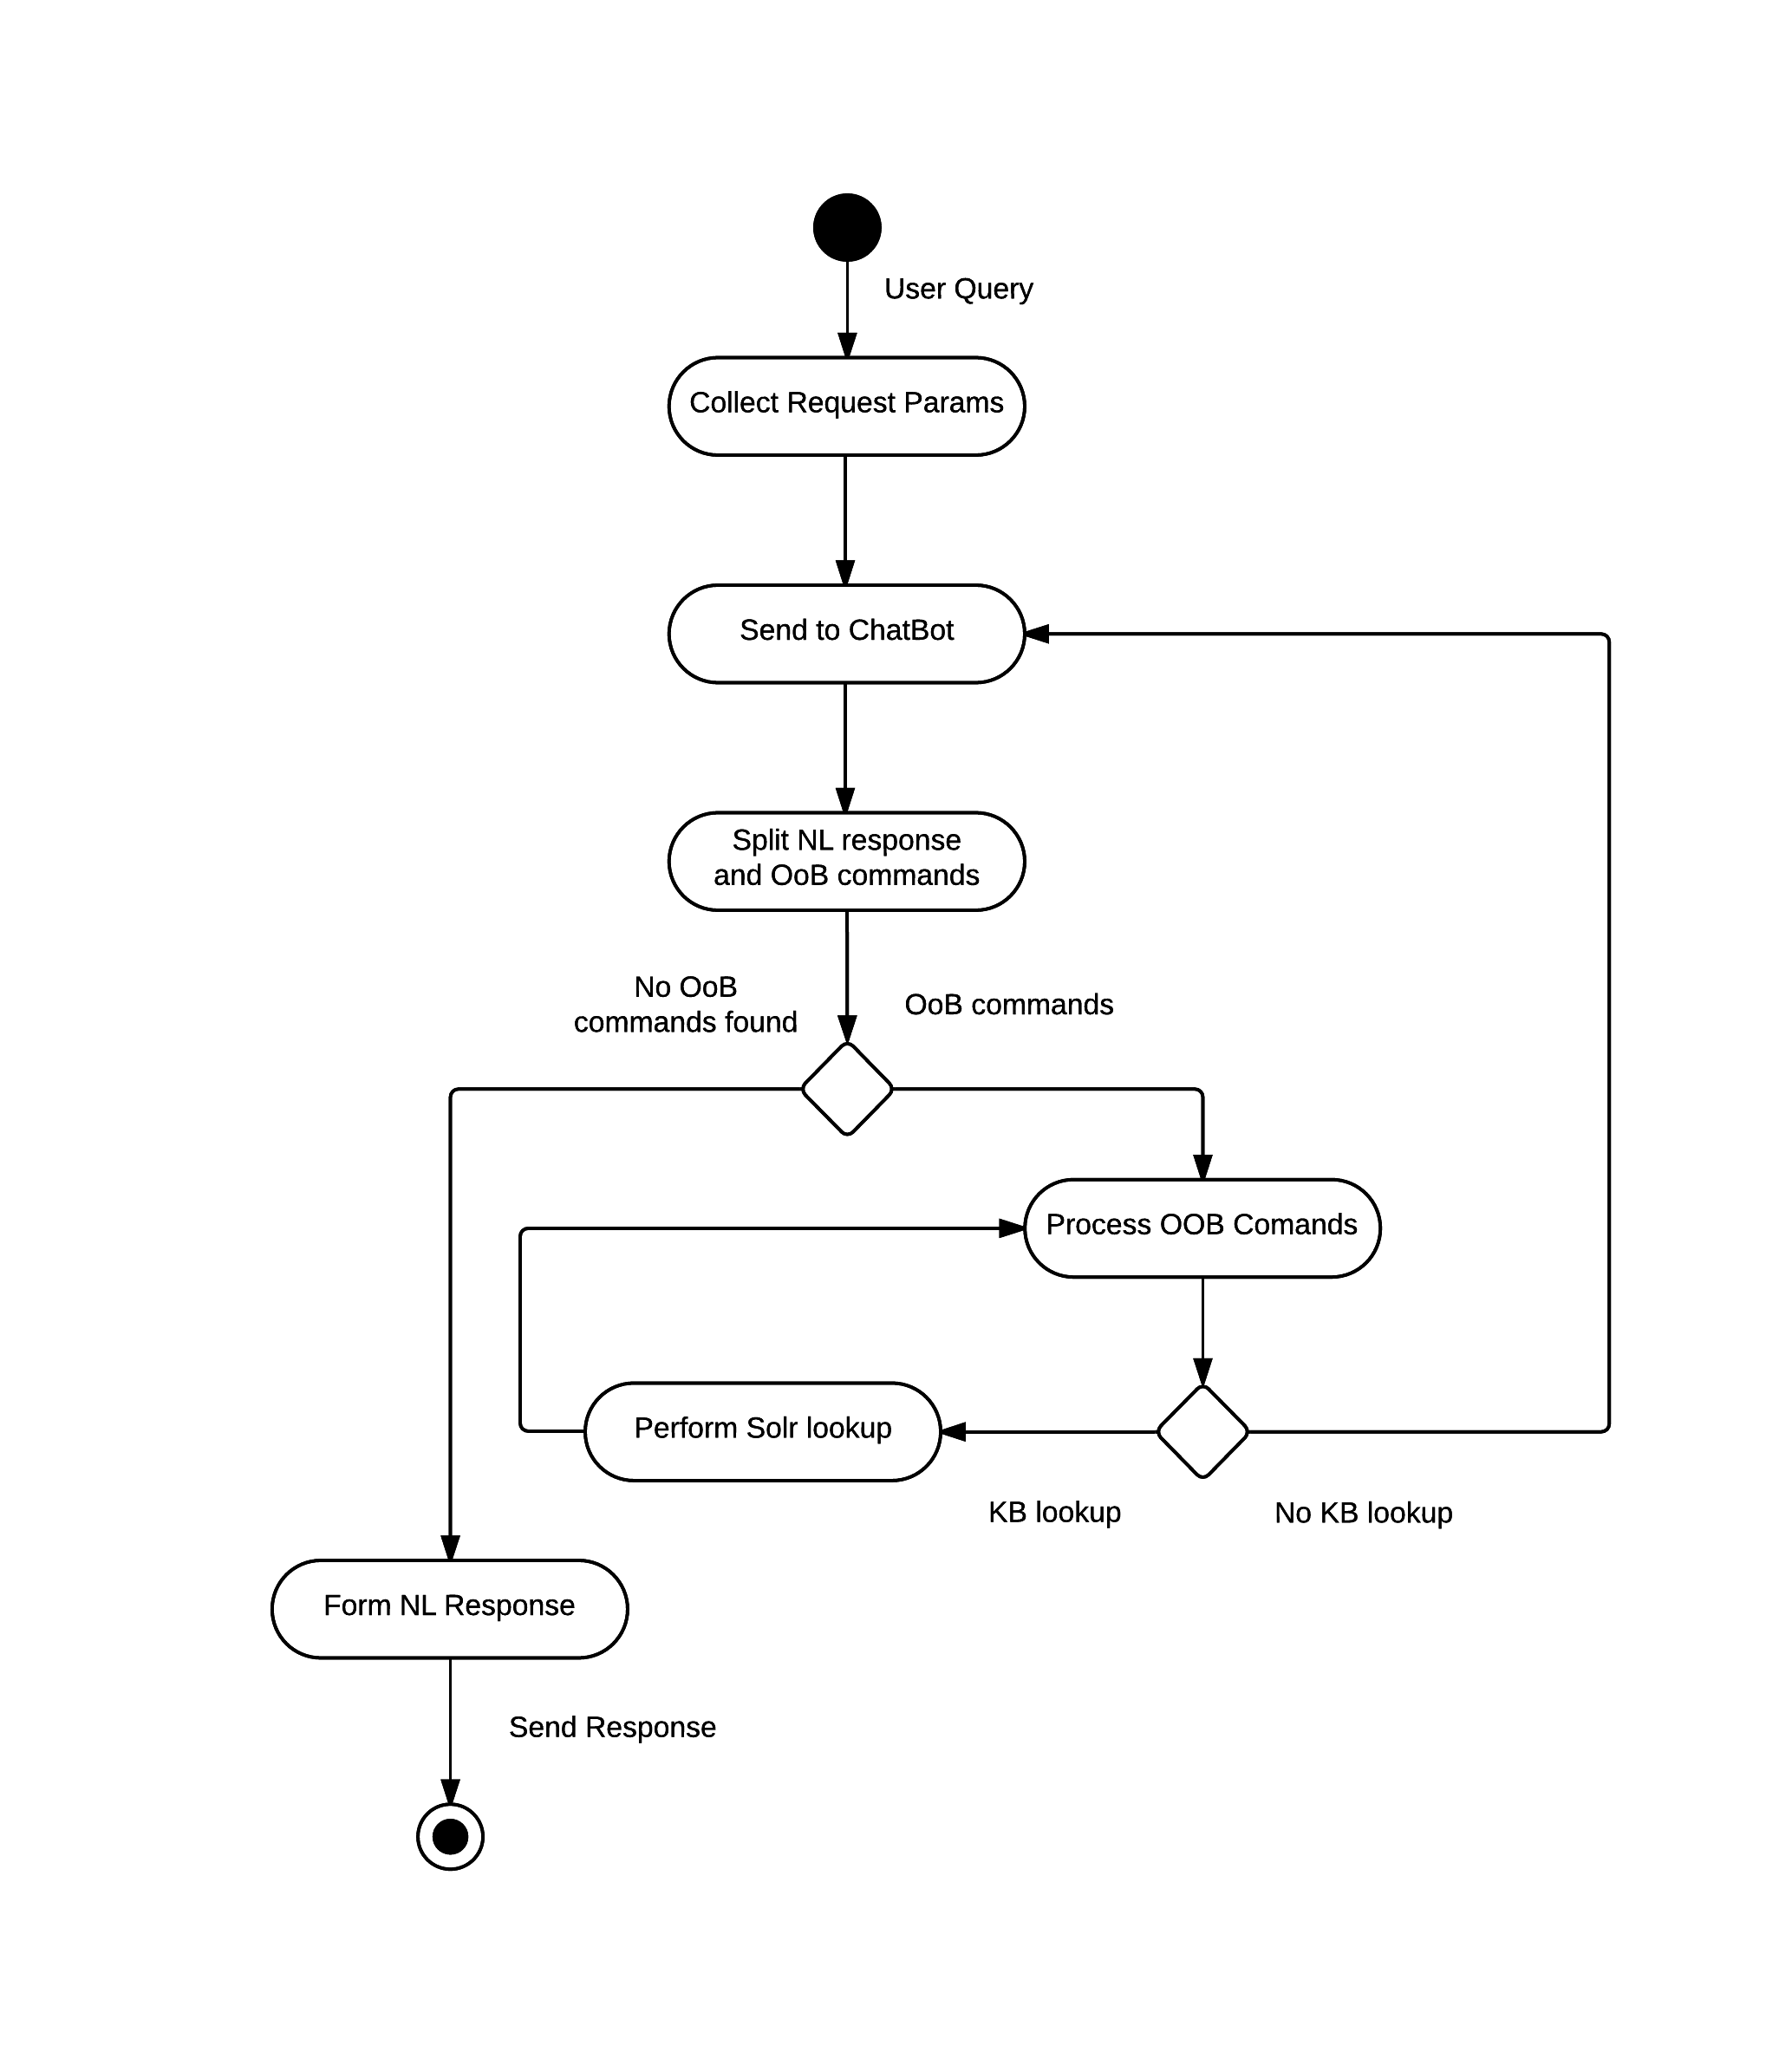
\includegraphics[width=0.6\textwidth]{img/prot/activityDiagram.png} % TODO: change this image for an actual UML diagram
    \caption{UML diagram of the process followed by the controller.}
    \label{fig:fe-model1}
\end{figure}

\begin{itemize}
 \item \textbf{Request parsing:} The client sends the query as JSON using a HTTP request to the fron-end controller. This JSON is recovered and processed into a python dictionary.
 \item \textbf{Send to ChatBot:} The user query is sent to the ChatBot so it's processes and a response, either \ac{NL} or \ac{OoB}, is generated.
 \item \textbf{Split \ac{NL} response and \ac{OoB} commands} The response in the previous step is split in \ac{NL} and {OoB} commands, to process each one appropriately.
 \item \textbf{\ac{OoB} command processing:} Read the \ac{OoB} commands and take the appropriate steps for each one of them.
 \item \textbf{Solr Lookup:} If a lookup in the Knowledge base is required, send the query to Solr.
 \item \textbf{Form Response:} Once there are no more \ac{OoB} commands, form the actual response in JSON and send it to the user.
\end{itemize}

% Add the workflow of the controller.

\subsubsection{Structural Model}

% Add functions in the askbot.py file and explain how they work

\subsection{ChatBot}

% Explain how chatscript works.

\subsection{Solr instance}

% Solr - add the relevant schema portions and how they work.

\section{Use cases}

% ¿? Something something... or something else?